\documentclass[parskip=full]{scrartcl}
\usepackage[top=2.54cm, bottom=2.54cm, left=2.54cm, right=2.54cm]{geometry}
\usepackage[utf8]{inputenc} % use utf8 file encoding for TeX sources
\usepackage[T1]{fontenc}    % avoid garbled Unicode text in pdf
\usepackage[ngerman]{babel}  % german hyphenation, quotes, etc
\usepackage{hyperref}
\usepackage{enumerate}
\usepackage[shortlabels]{enumitem}
\usepackage[dvipsnames]{xcolor}
\usepackage{graphicx}
\usepackage{mwe}
\usepackage{caption}
\usepackage{adjustbox}

% Set footer and header bar
\usepackage[headsepline, footsepline]{scrlayer-scrpage}
\addtokomafont{headsepline}{\color{BlueViolet}}
\addtokomafont{footsepline}{\color{BlueViolet}}
\KOMAoptions{headsepline=1.25pt:\textwidth}
\KOMAoptions{footsepline=1.25pt:\textwidth}
\clearpairofpagestyles
\rofoot{\thepage}
\ihead{Write your own Android App: Recishare}

\hypersetup{
    pdftitle={PSE: Pflichtenheft},
    colorlinks,
    linkcolor={black!50!black},
    citecolor={blue!50!black},
    urlcolor={blue!80!black}
}
\usepackage{csquotes}
% detailed hyperlink/pdf configuration
% ‘texdoc hyperref‘ for options
% provides \enquote{} macro for "quotes"


\begin{document}
\begin{titlepage}
    \begin{center}
        \begin{Huge}
            {\textbf{Write your own Android App: Recishare}}
        \end{Huge}
        \vspace{12px}

        Praxis der Softwareentwicklung (PSE)\\
        Sommersemester 2023\\
        \vspace{150px}

        \begin{Huge}
            {\textbf{Pflichtenheft}}
        \end{Huge}
        \vspace{12px}

        Auftraggeber\\
        Karlsruher Institut für Technologie\\
        KASTEL — Institut für Informationssicherheit und Verlässlichkeit\\
        \vspace{330px}

        Auftragnehmer\\
        Karlsruher Intellektuelle\\
        Henri Becker, Konrad Knappe, Lukas Schwarz, Raphael Zipperer\\
    \end{center}
\end{titlepage}

\tableofcontents

\vspace{32px}
\section*{Gender-Hinweis}
Zur besseren Lesbarkeit wird in diesem Pflichtenheft das generische Maskulinum verwendet.
Die in diesem Heft verwendeten Personenbezeichnungen beziehen sich – sofern nicht anders kenntlich gemacht – auf alle Geschlechter.
\newpage


\section{Zielbestimmung}

\subsection{Musskriterien}
Musskriterien: unabdingbare Leistungen der Software.

\begin{enumerate}[start=1,label={$\langle$\bfseries RM\arabic*$\rangle$}, leftmargin = 5em, itemsep=4pt, parsep=4pt]

    \item Die App besitzt eine Nutzerverwaltung.\label{RM1}
    \item Der Nutzer muss sich registrieren, einloggen und ausloggen können.\label{RM2}
    \item Der Nutzer muss eine Gruppe erstellen und diese auch wieder auflösen können.\label{RM3}
    \item Der Nutzer muss Gruppen einer Gruppe mithilfe eines Gruppenkürzels beitreten können und diese danach auch wieder verlassen können.\label{RM4}
    \item Es muss in jeder Gruppe mindestens ein Gruppenadmin sein.\label{RM5}
    \item Der Nutzer muss Rezepte erstellen und hochladen können.\label{RM6}
    \item Der Nutzer muss zu jedem Rezept den Rezepttitel, die Zubereitungsdauer, die Zutaten mit Mengenangaben, den Schwierigkeitsgrad, die Portionsanzahl und eine Zubereitungsanweisungen angeben können.\label{RM7}
    \item Es müssen erstellte Rezepte von anderen Nutzern in der gleichen Gruppe angeschaut werden können.\label{RM8}
    \item Ein erstellte Rezepte muss vom Autor separat verwaltet, geändert und gelöscht werden können.\label{RM9}
    \item Jedes Gruppenmitglied muss das Gruppenkürzel einsehen können.\label{RM10}
\end{enumerate}

\subsection{Sollkriterien}
Sollkriterien: erstrebenswerte Leistungen.

\begin{enumerate}[start=1,label={$\langle$\bfseries RS\arabic*$\rangle$}, leftmargin = 5em, itemsep=4pt, parsep=4pt]
    
    \item Der Nutzer soll bei Rezepten Portionen skalieren können.\label{RS1}
    \item Der Nutzer soll Rezepte favorisieren können.\label{RS2}
    \item Ein Admin soll weiter Gruppenmitglieder zum Admin ernennen können und jenen auch den Adminstatus wieder entziehen können.\label{RS3}
    \item Ein Admin soll Nutzer aus Gruppen kicken, bannen und auch wieder entbannen können.\label{RS4}
    \item Ein Admin soll Rezepte von Nutzern vor anderen Nutzern in der Gruppe ausblenden können.\label{RS5}
    \item Das Hinzufügedatum eines Rezeptes soll einsehbar sein.\label{RS7}
    \item Der Nutzer soll sein Passwort wieder zurücksetzen können.\label{RS8}
    \item Der Nutzer soll sein Konto nach erstellen wieder löschen können.\label{RS9}
    \item Der Nutzer soll das Gruppenkürzel auch über einen QR-Code teilen können.\label{RS10}
    \item Der Nutzer soll seinen Benutzernamen ändern können.\label{RS11}
\end{enumerate}

\subsection{Kannkriterien}
Kannkriterien: Leistungen, die enthalten sein können.

\begin{enumerate}[start=1,label={$\langle$\bfseries RC\arabic*$\rangle$}, leftmargin = 5em, itemsep=4pt, parsep=4pt]
    \item Der Nutzer kann Rezepte in Form von PDFs exportiert werden.\label{RC1}
    \item Der Nutzer kann zwischen Dark Mode und Light Mode wechseln können.\label{RC2}
    \item Der Nutzer kann genau ein Bild zum Rezept hochladen.\label{RC3}
    \item Der Nutzer kann Zutaten aus einer Liste auswählen.\label{RC4}
    \item Der Nutzer kann sein Profilbild ändern.\label{RC5}
    \item Der Nutzer kann Rezepte filtern nach Favoriten und Schwierigkeitsgrad.\label{RC6}
    \item Der Nutzer kann Rezepte jeweils auf- und absteigend sortieren Alphabetisch nach dem Namen des Rezepts, nach dem Schwierigkeitsgrad und dem Hinzufügedatum.\label{RC7}
    \item Ein Admin kann den Gruppennamen ändern.\label{RC8}
\end{enumerate}

\subsection{Abgrenzungskriterien}
Abgrenzungskriterien: Leistungen die explizit nicht umgesetzt werden.

\begin{enumerate}[start=1,label={$\langle$\bfseries RW\arabic*$\rangle$}, leftmargin = 5em, itemsep=4pt, parsep=4pt]
    \item Es können keine Kommentare zu Rezepten hinzugefügt werden.
    \item Der Nutzer kann keine Rezepte bewerten.
    \item Es gibt keine integrierte Chatfunktion.
    \item Es können keine Videos den Rezepten hinzugefügt werden.
    \item Es können keine Nutzer direkt über die App gesucht werden.
    \item Es existiert kein Gruppenprofilbild.
\end{enumerate}

\section{Produkteinsatz}
Dieses Kapitel dient dazu, den Einsatzbereich, die Zielgruppen und die Betriebsbedingungen der zu entwickelnden Software aufzuführen.

\subsection{Anwendungsbereiche}
In diesem Abschnitt wird erläutert, in welchen Bereichen die Software eingesetzt werden soll.
Die App bietet eine Reihe von Funktionen, die Nutzern eine Vielzahl an Anwendungsmöglichkeiten rund um das Thema kochen bieten. 
Zum einen können Nutzer Rezepte hochladen und diese bei Bedarf im Nachhinein bearbeiten. 
Diese Funktionen ermöglichen das Teilen von Rezepten mit anderen Nutzern. 
Zudem können sie als eine Art digitales Kochbuch benutzt werden, um eigene Rezepte zu organisieren und bei Bedarf auch von anderen Geräten aufrufen zu können. 
Außerdem können Nutzer die Rezepte anderer Nutzer betrachten, bewerten und speichern. 
Um zielgerichtet gewünschte Ergebnisse zu finden, gibt es eine Suchfunktion, mit der Nutzer Rezepte und andere Nutzer finden können. 
So können Nutzer gezielt ihre Kochkenntnisse erweitern. 
Rezepte können skaliert werden, um die richtige Menge für eine bestimmte Anzahl an Personen effizient zu ermitteln. 
Nutzer können außerdem Kochgruppen beitreten, um Rezepte mit Nutzern mit ähnlichen Interessen zu teilen. 
Die App ist explizit kein soziales Medium und besitzt dementsprechend keinerlei Chat- bzw. Kommentarsektionen.

\subsection{Zielgruppen}
Im Folgenden wird aufgezählt, für welche Anwender die Software im Wesentlichen gedacht ist. 
Die Kochapp richtet sich an alle, die gerne kochen und ihre Kocherfahrung verbessern möchten. 
Die App ist insbesondere für Gruppen geeignet, in denen gekocht wird (bsp. Wohngemeinschaften), da Rezepte effizient geteilt und skaliert werden können.

\subsection{Betriebsbedingungen}
In diesem Unterkapitel wird auf die unterschiedlichen Bedürfnisse und Anforderungen an die Software eingegangen.

\section{Produktübersicht}
In diesem Kapitel werden die Produktfunktionen beschrieben und in einem Use-Case-Diagramm visualisiert.
Das Use-Case-Diagramm zeigt mittels Verbindungslininen, wie die einzelnen Use-Cases zueinander stehen.
Der Abschnitt „Gruppenverwaltung“ und "Rezepte Liste" werden genauer in jeweils einem Aktivitätsdiagramm abgebildet.
Dadurch können die einzelnen Schritte, die durchlaufen werden, besser beschrieben werden.

\paragraph{Abbildung 3.1}
In dem Use-Case-Diagramm „Aufbau der App“ sieht man die allgemeine Struktur der App.\\
Bei der erstmaligen Nutzung muss der Nutzer sich registrieren.
Dazu muss er seinen Namen, seine E-Mail-Adresse und ein Passwort eingeben.
Das Passwort muss durch eine erneute Eingabe berstätigt werden.
Falls der Nutzer schon einen Nutzerkonto besitzt kann er sich einloggen.
Dazu muss er seine E-Mail-Adresse und sein Passwort eingeben.
Hat der Nutzer sein Passwort vergessen besteht die Möglichkeit das Passwort zurückzusetzen.
Ein eingeloggter Nutzer muss sich nicht erneut einloggen.\\
Nach dem Einloggen gelangt der Nutzer auf die Rezept-Ansicht.
Hier hat er die Möglichkeit, Rezepte zu filtern, suchen oder zu sortieren.
Durch klicken auf ein Rezept kann der Nutzer das Rezept ansehen, favorisieren und die Portionsgrößen ändern.\\
Durch klicken auf die Schaltfläche "Rezept erstellen" kann der Nutzer ein neues Rezept erstellen.
Es können Zutaten, Kochanleitung, Schwierigkeit und Kochzeit ƒür das neue Rezept angegeben werden.
Im Anschluss kann das Rezept veröffentlicht werden.\\
Durch klicken auf die Schaltfläche "Verwaltungs-Ansicht" gelangt der Nutzer auf die "Verwaltungs-Ansicht".
In dieser Ansicht kann der Nutzer sich ausloggen, sein Nutzerkonto löschen, seinen Nutzernamen ändern, 
erstellte Rezepte bearbeiten, eine Gruppe verlassen und Gruppen-Kürzel und das dazugehörige Passwort kopieren.\\
Durch das drücken der Schaltfläche "Gruppe hinzufügen" kann der Nutzer eine neue Gruppe erstellen oder beitreten.
Eine Gruppe kann durch Eingabe eines Gruppennamen und Passwort erstellt werden.\\ %Passiv
Von der Verwaltungsansicht-


\paragraph{Abbildung 3.2}
Im Aktivitätsdiagramm „Rezepte Liste“ werden die verschiedenen Möglichkeiten unter dem Menüpunkt aufgeführt.
Der Nutzer hat die Möglichkeite Rezepte durch eine Suchfeld zu suchen.
Der Nutzer hat die Möglichkeit die Rezepteliste durch vorgegebene Sortierungen zu sortieren.
Beim Auswählen eines Rezepts öffnet sich das zugehörige Rezeptfenster.
Im Rezeptfenster kann der Nutzer die Portionsgröße anpassen, das Rezept bewerten und das Rezept fovorisieren.
Im Fenster Rezeptliste kann der Nutzer Rezepte erstellen.
Es öffnet sich ein leeres Rezepttemplate Fenster.
Der Nutzer kann die Zutaten und die Kochanleitung in diesem Fenster eingeben.
Nach Bestätigung der Eingabe kommt der Nutzer wieder auf die Rezept Liste.

\paragraph{Abbildung 3.3}
Im Aktivitätsdiagramm Verwaltung  möchte der Nutzer seine Gruppen verwalten.
Es besteht die Wahl eine Gruppe zu erstellen, eine Gruppe hinzuzufügen oder bestehende Gruppen zu verwalten.
Beim erstellen einer Gruppe kann der Nutzer einen Gruppennamen und ein Passwort wählen.
Nach Bestätigung wird der Nutzer der Gruppe hinzugefügt.
Die Gruppe ist daraufhin unter Verwaltung zu finden.
Beim hinzufügen einer Gruppe muss der Nutzer das Gruppen-Kürzel und Passwort eingeben.
Bei erfolgreicher Eingabe wird der Nutzer der Gruppe hinzugefügt.
Bei fehlerhafter Eingabe erscheint eine Fehlermeldung.
Falls der Nutzer schon in einer Gruppe beigetreten ist, kann er der Gruppe austreten oder das Gruppen-Kürzel und Passwort der Gruppe kopieren.
Beim Austreten muss der Nutzer noch nachträglich bestätigen, dass er aus der austreten möchte.
\newpage

\begin{figure}[!htp]
    \centering
    \begin{adjustbox}{right=160mm}
        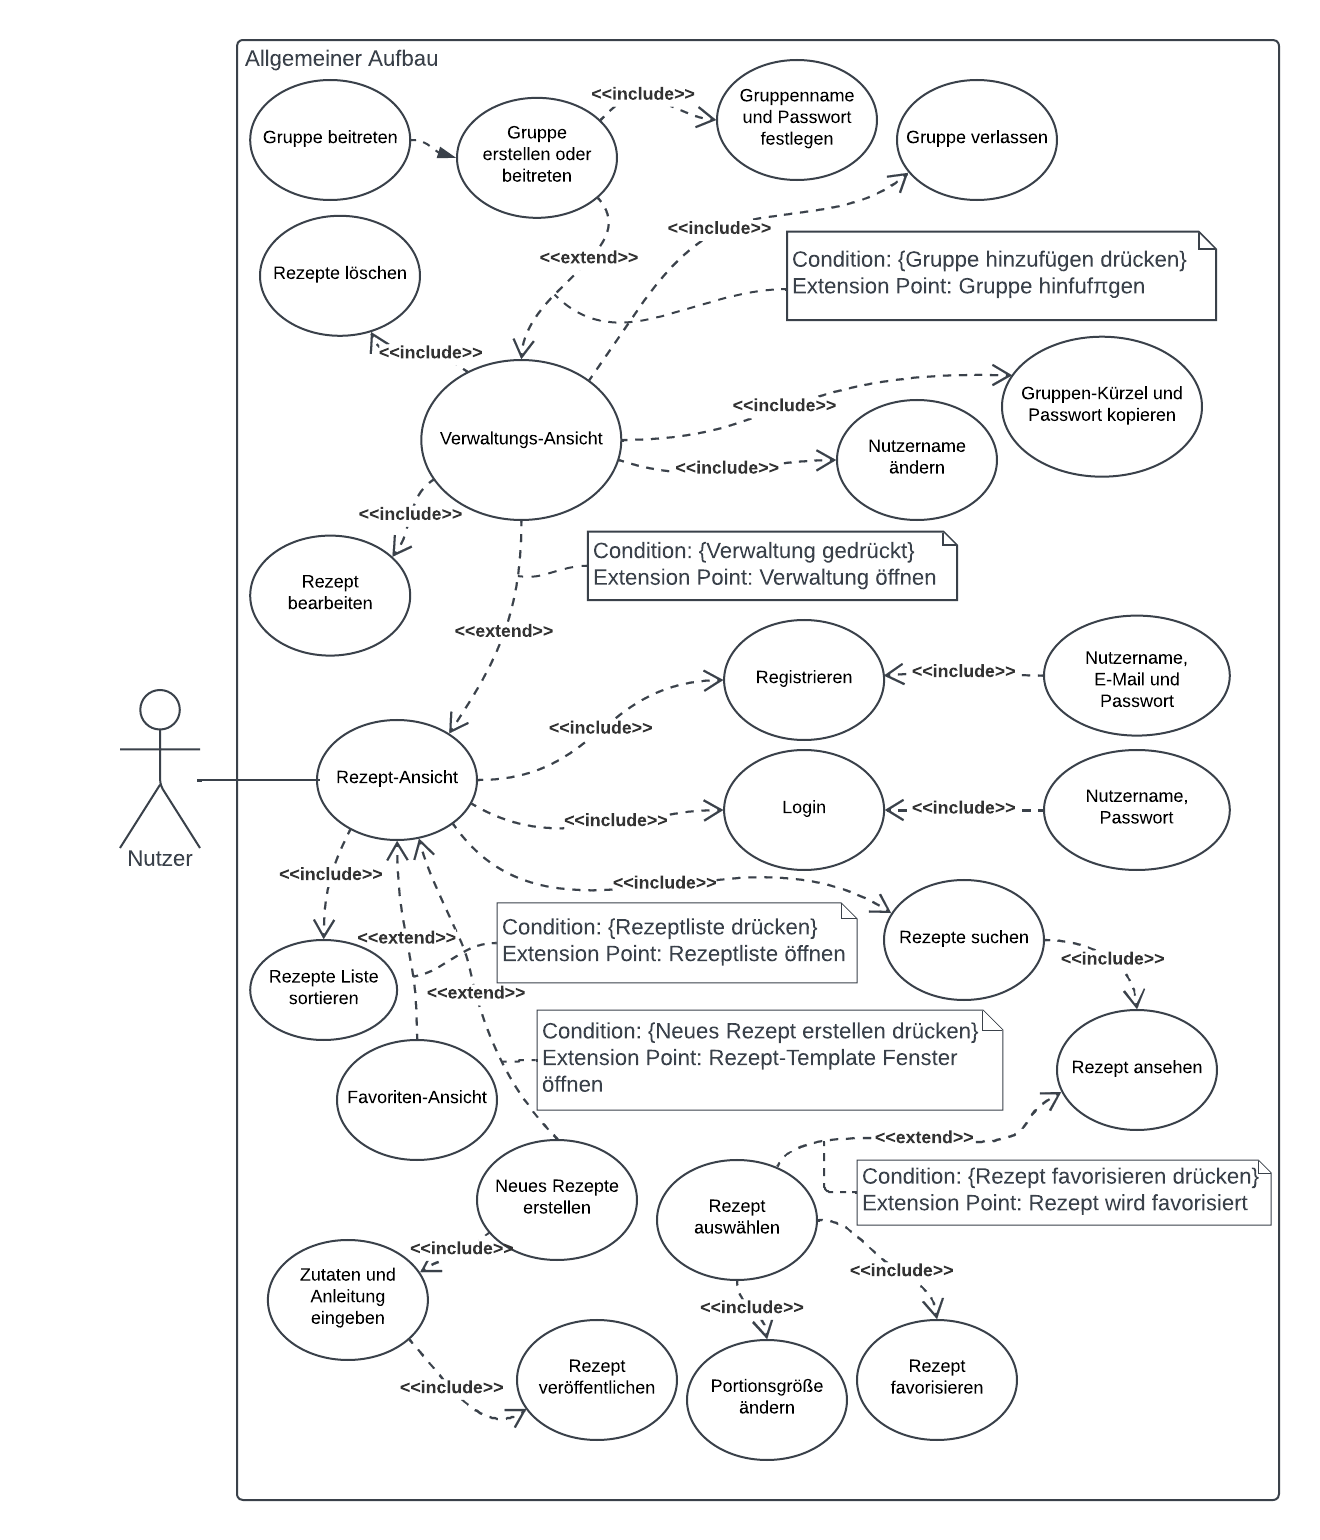
\includegraphics[height=220mm]{images/section3/Use-Case-Diagramm Aufbau App.png}
    \end{adjustbox}
    \caption*{Abbildung 3.1: Use-Case-Diagramm: Aufbau der App}
    \label{fig:A31}
\end{figure}
\newpage

\begin{figure}[!htp]
    \centering
    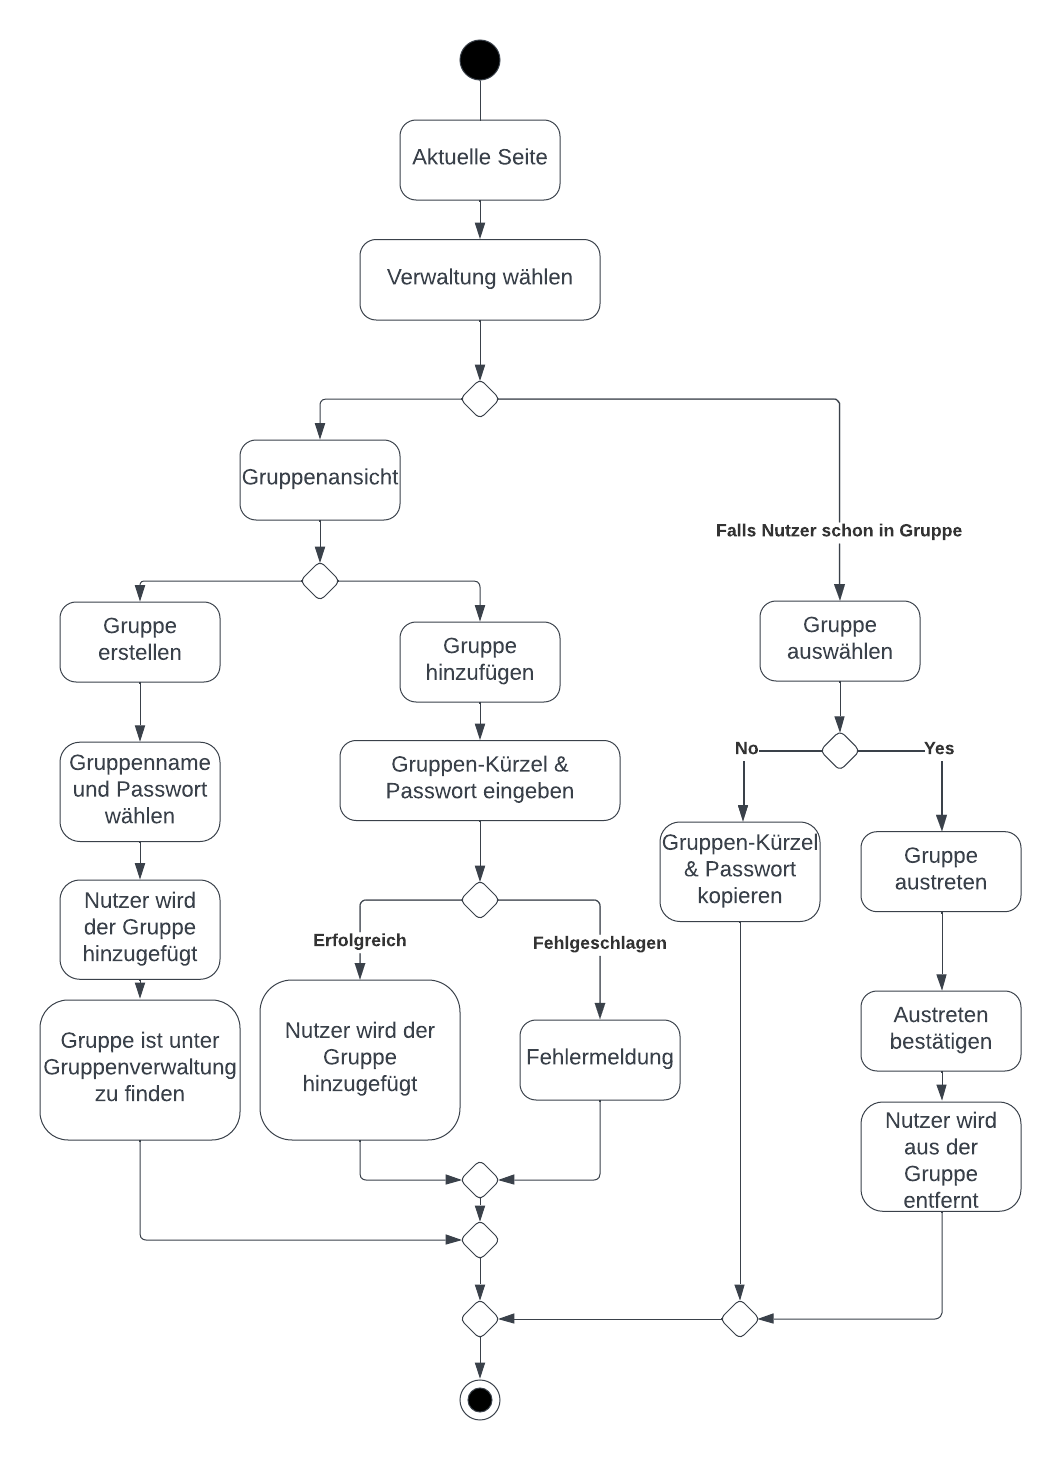
\includegraphics{images/section3/Aktivitaetsdiagramm Gruppenverwaltung.png}\\
    Abbildung 3.2: Aktivitätsdiagramm: Rezepte Liste
    \label{fig:A32}
\end{figure}
\newpage

\begin{figure}[!htp]
    \centering
    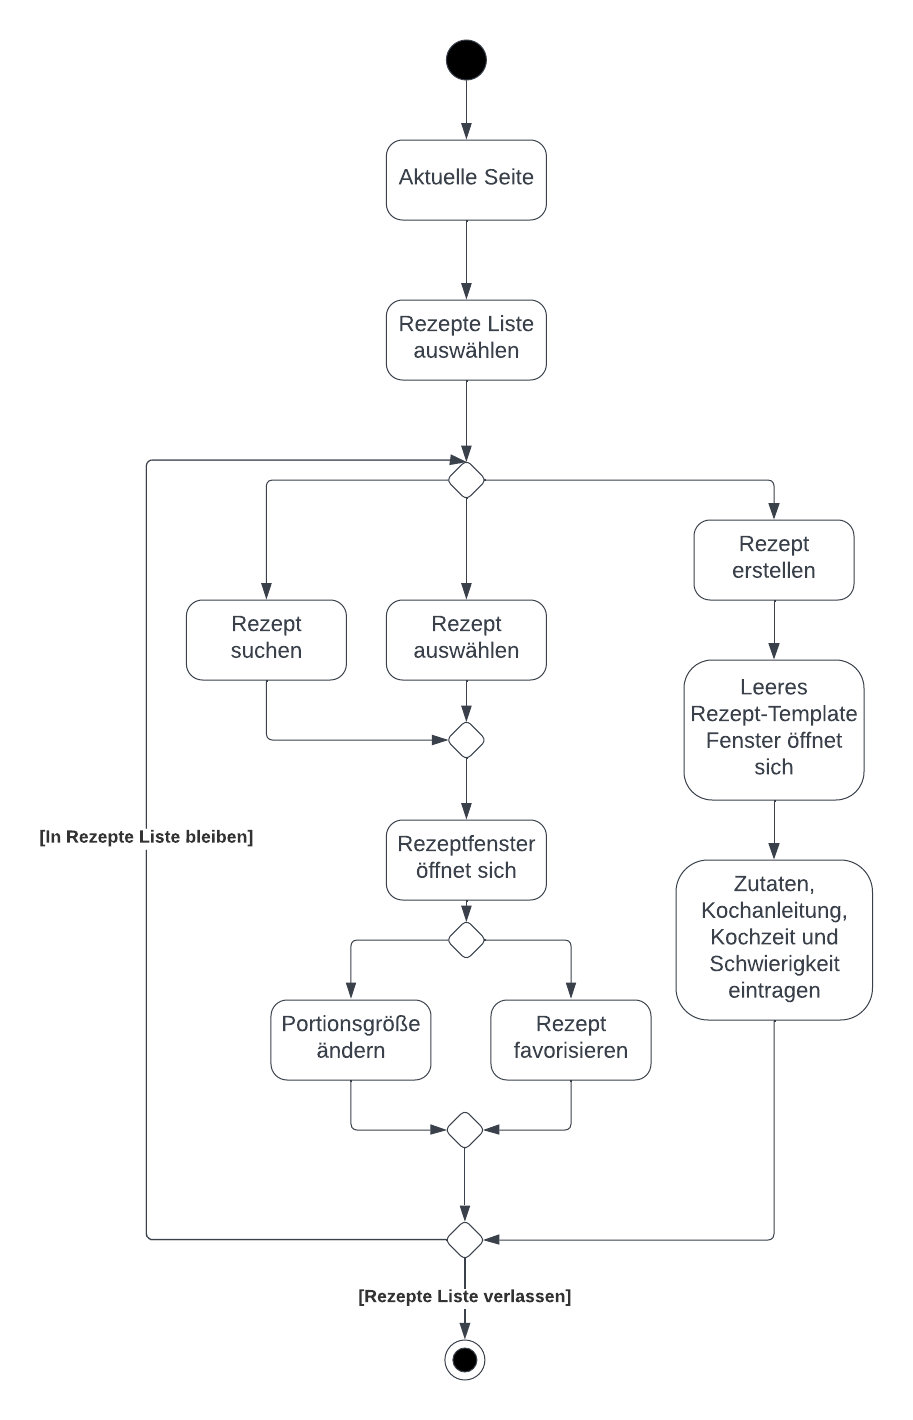
\includegraphics{images/section3/Aktivitaetsdiagramm Rezepte Liste.png}\\
    Abbildung 3.3: Aktivitätsdiagramm: Gruppenverwaltung
    \label{fig:A33}
\end{figure}
\newpage

\section{Produktfunktion}
\textbf{Einloggen und Ausloggen $\langle$F10$\rangle$}\\
\textbf{Anwendungsfall:} Der Nutzer möchte sich in der App anmelden und sich danach wieder ausloggen.\\
\textbf{Anforderungen:} \ref{RM1}, \ref{RM2}\\
\textbf{Ziel:} Der Nutzer erhält Zugang zu seinem Profil in der App, indem eine Verbindung zum Server hergestellt wird. Danach wird diese Verbindung wieder getrennt\\
\textbf{Vorbedingung:} Der Nutzer hat bereits ein Konto erstellt.\\
\textbf{Nachbedingung Erfolg:} Der Nutzer ist erfolgreich ausgeloggt und wird zur Login-Ansicht der App weitergeleitet.\\
\textbf{Nachbedingung Fehlschlag:} Das Passwort oder der Nutzername ist falsch, sodass eine Fehlermeldung erscheint bei dem fehlerhaften Eingabefeld.\\
\textbf{Akteure:} Nutzer, Server\\
\textbf{Auslösendes Ereignis:} -\\
\textbf{Beschreibung:}
\begin{enumerate}
    \item Der Nutzer startet die App.
    \item Die Login-Ansicht erscheint
    \item Der Nutzer gibt seinen Nutzernamen ein.
    \item Der Nutzer gibt sein Passwort ein.
    \item Der Nutzer klickt auf den Weiter-Button, um die Anmeldung abzuschließen.
    \item Der Nutzer klickt auf den Verwaltungs-Ansichts-Button.
    \item Der Nutzer Klick auf den ausloggen-Button.
    \item Der Nutzer wird zur Login-Ansicht weitergeleitet
\end{enumerate}
\textbf{Erweiterung:} -\\
\textbf{Alternativen:} Mit einem Klick auf den Registrieren-Button kann ein Nutzer Konto angelegt werden. Mit einem Klick auf den Passwort-vergessen-Button Knopf kann das Passwort eines bestehenden Kontos geändert werden.  \\
\newpage


\textbf{Registrierung und Konto löschen $\langle$F20$\rangle$}\\
\textbf{Anwendungsfall:} Der Nutzer möchte ein Nutzerkonto anlegen und danach sein Konto löschen.\\
\textbf{Anforderungen:} \ref{RM2}, \ref{RS8} \\
\textbf{Ziel:} Der Nutzer legt ein Nutzerkonto an, um alle Features der App nutzen zu können und löscht das Nutzerkonto danach.\\
\textbf{Vorbedingung:} -\\
\textbf{Nachbedingung Erfolg:} Der Nutzer wird zum Gruppen-Ansicht weitergeleitet und mit einem Pop-up-Fenster erfolgt die Bestätigung zur erfolgreichen Registrierung.\\
\textbf{Nachbedingung Fehlschlag:} Eine Fehlermeldung erscheint beim fehlerhaften Eingabefenster.\\
\textbf{Akteure:} Nutzer, Server\\
\textbf{Auslösendes Ereignis:} Der Nutzer muss auf den Registrieren-Button in der Login-Ansicht klicken.\\
\textbf{Beschreibung:}
\begin{enumerate}
    \item Der Nutzer klickt auf den Registrieren-Button.
    \item Der Nutzer gibt einen Nutzernamen ein.
    \item Der Nutzer gibt seine E-Mail-Adresse ein.
    \item Der Nutzer gibt ein Passwort ein.
    \item Der Nutzer gibt das Passwort nochmals ein.
    \item Der Nutzer klickt auf den Weiter-Button.
    \item Der Nutzer wird zur Login-Ansicht weitergeleitet.
    \item Der Nutzer klickt auf den Verwaltungs-Ansichts-Button.
    \item Der Nutzer klickt auf den Konto-Löschen-Button.
    \item Ein Pop-up-Fenster erscheint zur Bestätigung zum Löschen des Benutzerkonto löschen.
    \item Der Nutzer klickt auf den Bestätigen-Button.
    \item Das Benutzerkonto wird gelöscht.
    \item der Nutzer wird zur Login-Ansicht weitergeleitet.
\end{enumerate}
\textbf{Erweiterung:} -\\
\textbf{Alternativen:} -\\
\newpage


\textbf{Passwort zurücksetzen $\langle$F20$\rangle$}\\
\textbf{Anwendungsfall:} Der Nutzer möchte das Passwort für seinen Benutzerkonto zurücksetzen.\\
\textbf{Anforderungen:} \ref{RS7}\\
\textbf{Ziel:} Der Nutzer kann ein neues Passwort setzen.\\
\textbf{Vorbedingung:} Die App muss bereits gestartet worden sein.\\
\textbf{Nachbedingung Erfolg:} Der Nutzer wird zum Login-Ansicht weitergeleitet und mit einem Pop-up-Fenster erfolgt die Bestätigung der Versendung einer E-Mail an die angegeben E-Mail-Adresse.\\
\textbf{Nachbedingung Fehlschlag:} Ein Pop-up-Fenster erscheint mit einer Fehlermeldung.\\
\textbf{Akteure:} Nutzer, Server\\
\textbf{Auslösendes Ereignis:} Der Nutzer muss auf den Passwort-vergessen-Button in der Login-Ansicht klicken.\\
\textbf{Beschreibung:}
\begin{enumerate}
    \item Klick auf den Passwort-vergessen-Button.
    \item Eingabe der E-Mail-Adresse.
    \item Klick auf den Weiter Button.
\end{enumerate}
\textbf{Erweiterung:} -\\
\textbf{Alternativen:} Durch das Klicken auf den Verlassen Button wird der Nutzer zurück zur Login-Ansicht geleitet.\\
\newpage


\textbf{Benutzernamen und Profilbild ändern $\langle$F30$\rangle$}\\
\textbf{Anwendungsfall:} Der Nutzer möchte seinen Benutzernamen und sein Profilbild ändern.\\
\textbf{Anforderungen:} \ref{RS10}, \ref{RC5}\\
\textbf{Ziel:} Der Nutzer kann seinen Benutzernamen und sein Profilbild an seine Wünsche anpassen.\\
\textbf{Vorbedingung:} -\\
\textbf{Nachbedingung Erfolg:} Der aktualisierte Nutzername und das aktualisierte Profilbild wird anderen Nutzern angezeigt.\\
\textbf{Nachbedingung Fehlschlag:} Ein Pop-up-Fenster erscheint mit einer Fehlermeldung.\\
\textbf{Akteure:} Nutzer, Server\\
\textbf{Auslösendes Ereignis:} Der Nutzer klickt auf den Button für die Verwaltungs-Ansicht.\\
\textbf{Beschreibung:}
\begin{enumerate}
    \item Der Nutzer klickt auf den Button für die Verwaltungs-Ansicht.\\
    \item Der Nutzer klickt auf den Nutzernamen bearbeiten Button.
    \item Der neue Benutzername wird eingegeben.
    \item Der Nutzer klickt auf den speichern Button.
    \item Der Nutzer klickt auf sein Profilbild.
    \item Der Nutzer kann mit Hilfe des betriebssystemeigenen Dateimanagers ein neues Profilbild aussehen.
\end{enumerate}
\textbf{Erweiterung:} -\\
\textbf{Alternativen:} Der Nutzer kann auch sein Profilbild komplett entfernen. Auch kann der Nutzer auf den Exit Button klicken und der Prozess wird abgebrochen und der Nutzer gelangt zurück zur Verwaltungs-Ansicht.\\
\newpage



\textbf{Rezept erstellen, ändern und löschen$\langle$F40$\rangle$}\\
\textbf{Anwendungsfall:} Der Nutzer möchte ein neues Rezept erstellen, es danach ändern und es schließlich löschen.\\
\textbf{Anforderungen:} \ref{RM6}, \ref{RM7}, \ref{RM9}, \ref{RC3}, \ref{RC4}\\
\textbf{Ziel:} Der Nutzer erstellt ein Rezept, welches er mit seinen Gruppen teilen möchte, oder auch nur für sich sichtbar macht. Nimmt dann Änderungen vor, um es dann wieder zu löschen.\\
\textbf{Vorbedingung:} -\\
\textbf{Nachbedingung Erfolg:} Das erstellte und geänderte Rezept wird in der Verwaltungs-Ansicht nicht mehr angezeigt.  \\
\textbf{Nachbedingung Fehlschlag:} Ein Pop-up-Fenster erscheint mit einer Fehlermeldung.\\
\textbf{Akteure:} Nutzer, Server\\
\textbf{Auslösendes Ereignis:} In der Haupt-Ansicht klickt der Nutzer auf den neues-Rezept -anlegen-Button.\\
\textbf{Beschreibung:}
\begin{enumerate}
    \item Der Nutzer klickt auf den Button für ein neues Rezept.
    \item Der Nutzer gib den Rezepttitel, die Zubereitungsdauer, die Zutaten mit Mengenangaben, den Schwierigkeitsgrad, die Portionsanzahl und eine Zubereitungsanweisungen an.
    \item Der Nutzer klickt auf den speichern Button.
    \item Der Nutzer wird zur Haupt-Ansicht weitergeleitet.
    \item Der Nutzer klickt auf den Verwaltungs-Ansicht Button.
    \item Der Nutzer klickt auf das gerade erstellte Rezept.
    \item Der Nutzer wird zur Rezept-erstellen-Ansicht weitegeleitet.
    \item Der Nutzer ändert den Rezepttitel.
    \item Der Nutzer klickt auf den Speichern Button.
    \item Der Nutzer wird zur Haupt-Ansicht weitergeleitet. 
    \item Der Nutzer klickt auf den Verwaltungs-Ansicht Button.
    \item Der Nutzer klickt auf den Löschen Button des gerade geänderten Rezepts.
    \item Ein Pop-up-Fenster erscheint mit der Frage zur Bestätigung, dass das Rezept gelöscht werden soll.
    \item Der Nutzer klickt auf den bestätigen Button.
    \item Dem Nutzer wird das Rezept nicht mehr angezeigt.
\end{enumerate}
\textbf{Erweiterung:} Der Nutzer kann ein Bild vom fertigen Gericht können.\\
\textbf{Alternativen:} -\\
\newpage

\textbf{Rezept suchen, sortieren, filtern, anschauen und favorisieren $\langle$F60$\rangle$}\\
\textbf{Anwendungsfall:} Der Nutzer möchte nach einem Rezept Suchen, dann die Rezepte nach dem Schwierigkeitsgrad filtern, ein Rezept sich genauer anschauen und dies dann favorisieren.\\
\textbf{Anforderungen:} \ref{RM8}, \ref{RS1}, \ref{RS2}, \ref{RC6}, \ref{RC7}, \ref{RC1} \\
\textbf{Ziel:} Der Nutzer kann mit dem Suchen, dem Filtern und dem Favorisieren sein gewünschtes Rezept schnell finden und es mithilfe der Zubereitungsanweisungen nachvollziehen.\\
\textbf{Vorbedingung:} Dem Nutzer wird mindestens ein Rezept in der Haupts-Ansicht oder in der Gruppen-Detail-Ansicht angezeigt.\\
\textbf{Nachbedingung Erfolg:} Das Rezept favorisierte Rezept ist mit den anderen favorisierten Rezepten beim Filter favorisierte Rezepte auffindbar.\\
\textbf{Nachbedingung Fehlschlag:} Ein Pop-up-Fenster erscheint mit einer Fehlermeldung.\\
\textbf{Akteure:} Nutzer, Server\\
\textbf{Auslösendes Ereignis:} Klick auf die Suchzeile in der Haupt-Ansicht.\\
\textbf{Beschreibung:}
\begin{enumerate}
    \item Der Nutzer klickt auf die Suchzeile.
    \item Der Nutzer gibt einen Suchbegriff ein.
    \item Der Nutzer klickt auf den Sortierungs-methode-Button und wählt Hinzufügedatum aus.
    \item Der Nutzer klickt auf den Filtern-nach-Button und wählt Schwierigkeitsgrad Mittel.
    \item Der Nutzer klickt auf ein Rezept.
    \item Der Nutzer wird zur Rezept-Ansicht weitergeleitet.
    \item Der Nutzer skaliert das Rezept auf eine Person.
    \item Der Nutzer klickt auf den Favoriten-Button.
\end{enumerate}
\textbf{Erweiterung:} Der Nutzer kann die voreingestellte Portionsgröße auf die gewünschte Anzahl ändern. Des Weiter kann ein Rezept auch in der Form eines PDFs exportiert werden.\\
\textbf{Alternativen:} -\\
\newpage


\textbf{Gruppe erstellen und Gruppe auflösen $\langle$F90$\rangle$}\\
\textbf{Anwendungsfall:} Der Nutzer möchte eine neue Gruppe erstellen, mit der die Rezepte geteilt werden können und diese danach wieder auflösen.\\
\textbf{Anforderungen:} \ref{RM3}, \ref{RM5} \\
\textbf{Ziel:} Der Nutzer kann mit der neuen Gruppe seine Rezepte teilen und danach die Gruppe auch wieder auflösen.\\
\textbf{Vorbedingung:} -\\
\textbf{Nachbedingung Erfolg:} Die erstellte Gruppe wird in der Verwaltung-Ansicht nicht mehr angezeigt und der Admin Status des Nutzers wird wieder entfernt.\\
\textbf{Nachbedingung Fehlschlag:} Ein Pop-up-Fenster erscheint mit einer Fehlermeldung.\\
\textbf{Akteure:} Nutzer, Server\\
\textbf{Auslösendes Ereignis:} Der Nutzer klickt auf den Gruppe-erstellen Button.\\
\textbf{Beschreibung:}
\begin{enumerate}	
    \item Der Nutzer klickt auf den Gruppe-erstellen Button.
    \item Der Nutzer wird zur Gruppen-Erstellungs-Ansicht weitergeleitet.
    \item Der Nutzer gibt den Gruppennamen ein.
    \item Der Nutzer klickt auf den speichern Button.
    \item Der Nutzer wird zur Verwaltungs-Ansicht zurückgeleitet.
    \item Der Nutzer klickt auf die Gruppe und wird zur Gruppen-Detail-Ansicht weitergeleitet.
    \item Der Nutzer klickt auf den Gruppen-auflösen-Button.
    \item Ein Pop-up-Fenster erscheint, welches um Bestätigung bitten.
    \item Der Nutzer klickt auf den Button zum Bestätigen.
\end{enumerate}
\textbf{Erweiterung:} -\\
\textbf{Alternativen:} Mit dem Gruppe-beitreten-Button kann auch zur Gruppen-Erstellungs-Ansicht gelangt werden.\\
\newpage

\textbf{Gruppe beitreten und verlassen $\langle$F100$\rangle$}\\
\textbf{Anwendungsfall:} Der Nutzer möchte einer neuen Gruppe beitreten und diese danach verlassen.\\
\textbf{Anforderungen:} \ref{RM4} \\
\textbf{Ziel:} Der Nutzer ist der Gruppe beigetreten und kann alle in der Gruppe geteilten Rezepte ansehen und diese auch wieder verlassen, sodass in der Haupt-Ansicht die Rezepte nicht mehr angezeigt werden.\\
\textbf{Vorbedingung:} -\\
\textbf{Nachbedingung Erfolg:} Die beigetretene Gruppe wird nicht mehr in der Verwaltung-Ansicht angezeigt und die Rezepte der Gruppe werden nicht mehr in der Haupt-Ansicht angezeigt.\\
\textbf{Nachbedingung Fehlschlag:} Ein Pop-up-Fenster erscheint mit einer Fehlermeldung.\\
\textbf{Akteure:} Nutzer, Server\\
\textbf{Auslösendes Ereignis:} Klick auf den Gruppe-beitreten Button.\\
\textbf{Beschreibung:}\\
\begin{enumerate}
    \item Der Nutzer klickt auf den Gruppe-beitreten-Button in der Verwaltung-Ansicht.
    \item Der Nutzer gibt das Gruppenkürzels ein.
    \item Der Nutzer klickt auf den Gruppe-beitreten-Button.
    \item Der Nutzer wird zur Gruppen-Detail-Ansicht weitergeleitet.
    \item Der Nutzer klickt auf den Gruppe-verlassen Button.
    \item Ein Pop-up-Fenster erscheint, welches um Bestätigung bitten.
    \item Der Nutzer klickt auf den Button zum Bestätigen.
    \item der Nutzer wird zur Verwaltungs-Ansicht weitergeleitet.
\end{enumerate}
\textbf{Erweiterung:} Mit dem Scannen eines QR-Codes kann auch einer Gruppe beigetreten werden ohne die Eingabe eines Gruppennamens.\\
\textbf{Alternativen:} Nach dem Login-Ansicht wird man zur Gruppe-beitreten-Ansicht weitergeleitet, wodurch auch einer Gruppe beigetreten werden kann.\\
\newpage

\textbf{Gruppenkürzel ausgeben $\langle$F120$\rangle$}\\
\textbf{Anwendungsfall:} Der Nutzer möchte den Gruppenkürzel erhalten.\\
\textbf{Anforderungen:} \ref{RM10}\\
\textbf{Ziel:} Der Nutzer kann die Daten der Gruppe mit anderen Nutzern teilen, um diese die Möglichkeit zu geben der Gruppe beizutreten.\\
\textbf{Vorbedingung:} Der Nutzer ist in einer Gruppe Mitglied.\\
\textbf{Nachbedingung Erfolg:} Ein Pop-up-Fenster erscheint mit den Daten der Gruppe.\\
\textbf{Nachbedingung Fehlschlag:} Ein Pop-up-Fenster erscheint mit einer Fehlermeldung.\\
\textbf{Akteure:} Nutzer, Server \\
\textbf{Auslösendes Ereignis:} Der Nutzer klickt in der Verwaltungs-Ansicht auf die Gruppe und wird zur Gruppen-Detail-Ansicht weitergeleitet.\\
\textbf{Beschreibung:}
\begin{enumerate}
    \item Der Nutzer klickt auf die Gruppen-Detail-Ansicht-Button.
    \item Der Nutzer klickt auf den Gruppen-Informations-Button.
    \item Der Nutzer wird zur QR-Code-Ansicht weitergeleitet.
    \item Der Nutzer sieht den QR-Code, der alle Informationen enthält.
\end{enumerate}
\textbf{Erweiterung:} -\\
\textbf{Alternativen:} -\\
\newpage


\textbf{Admin ernennen und Admin Status entfernen $\langle$F140$\rangle$}\\
\textbf{Anwendungsfall:} Der Nutzer möchte ein weiteres Mitglied der Gruppe zu einem Admin der Gruppe ernennen und dem Nutzer den Admin Status dann wieder aberkennen.\\
\textbf{Anforderungen:} \ref{RS3}\\
\textbf{Ziel:} Der Nutzer kann seine Rechte für die Gruppe mit anderen Mitgliedern teilen und auch anderen Mitglieder die Rechte entziehen.\\
\textbf{Vorbedingung:} Der Nutzer ist Admin der Gruppe.\\
\textbf{Nachbedingung Erfolg:} Ein weiteres Mitglied besitze die gegebenen Reche nicht mehr.\\
\textbf{Nachbedingung Fehlschlag:} Ein Pop-up-Fenster erscheint mit einer Fehlermeldung.\\
\textbf{Akteure:} Nutzer, Server \\
\textbf{Auslösendes Ereignis:} Klick auf die Detail-Ansicht eines Mitglieds der Gruppe.\\
\textbf{Beschreibung:}
\begin{enumerate}
    \item Der Nutzer klickt auf die Detail-Ansicht eines Mitglieds der Gruppe.
    \item Der Nutzer klickt auf die Option den Nutzer zum Admin der Gruppe zu ernennen.
    \item Ein Pop-up-Fenster erscheint mit einer Bestätigung, dass der Nutzer zum Admin der Gruppe ernannt wurde.
    \item Der Nutzer klickt auf die Detail-Ansicht eines Mitglieds der Gruppe.
    \item Der Nutzer klickt auf die Option den Nutzer die Admin Rechte der Gruppe zu entziehen.
     \item Ein Pop-up-Fenster erscheint mit einer Bestätigung, dass dem Nutzer die Admin Rechte entzogen worden.
\end{enumerate}
\textbf{Erweiterung:} -\\
\textbf{Alternativen:} -\\
\newpage

\textbf{Nutzer kicken und Nutzer bannen $\langle$F150$\rangle$}\\
\textbf{Anwendungsfall:} Ein Admin möchte ein Mitglied der Gruppe aus der Gruppe kicken und ein anderes Mitglied aus der Gruppe bannen und danach wieder entbannen.\\
\textbf{Anforderungen:} \ref{RS4}\\
\textbf{Ziel:} Ein Admin möchte das erste Mitglied nur aus der Gruppe kicken und dem zweiten Mitglied nicht mehr die Möglichkeit bieten der Gruppe beizutreten.\\
\textbf{Vorbedingung:} Der Nutzer ist Admin der Gruppe und die Gruppe hat insgesamt mindestens drei Mitglieder.\\
\textbf{Nachbedingung Erfolg:} Die beiden Nutzer sind nicht mehr in der Gruppe.\\
\textbf{Nachbedingung Fehlschlag:} Ein Pop-up-Fenster erscheint mit einer Fehlermeldung.\\
\textbf{Akteure:} Nutzer, Server \\
\textbf{Auslösendes Ereignis:} Der Nutzer klickt auf die Detail-Ansicht des Mitglieds der Gruppe.\\
\textbf{Beschreibung:}
\begin{enumerate}
    \item Der Nutzer klickt auf die Detail-Ansicht des ersten Mitglieds der Gruppe.
    \item Der Nutzer klickt auf die Option den Nutzer zu kicken.
    \item Ein Pop-up-Fenster erscheint mit einer Bitte um Bestätigung, dass der Nutzer gekickt werden soll.
    \item Der Nutzer klickt auf den Bestätigen-Button.
    \item Der Nutzer klickt auf die Detail-Ansicht des zweiten Mitglieds der Gruppe.
    \item Der Nutzer klickt auf die Option den Nutzer zu bannen.
    \item Der Nutzer klickt auf die Detail-Ansicht des gebannten Nutzers in der Liste der gebannten Nutzer.
    \item Der Nutzer klickt auf die Option den Nutzer zu entbannen.
    \item Ein Pop-up-Fenster erscheint mit einer Bitte um Bestätigung, dass der Nutzer entbannt werden soll.
    \item Der Nutzer klickt auf den Bestätigen-Button.
\end{enumerate}
\textbf{Erweiterung:} -\\
\textbf{Alternativen:} -\\
\newpage


\textbf{Rezepte verwalten für die Gruppen $\langle$F160$\rangle$}\\
\textbf{Anwendungsfall:} Der Nutzer will ein Rezept, welches mit der Gruppe von einem Nutzer geteilt wird, ausblenden und danach die Ausblendung wieder rückgängig machen.\\
\textbf{Anforderungen:} \ref{RS5}\\
\textbf{Ziel:} Der Nutzer kann bestimmen welche Rezepte den Mitgliedern und ihm selbst angezeigt werden.\\
\textbf{Vorbedingung:} Der Nutzer ist Admin der Gruppe und in der Gruppe bestehen Rezepte.\\
\textbf{Nachbedingung Erfolg:} Das Rezept wird wieder Hauptansicht oder in der Gruppen-Detail-Ansicht angezeigt nach dem es für die Mitglieder  ausgeblendet war.\\
\textbf{Nachbedingung Fehlschlag:} Ein Pop-up-Fenster erscheint mit einer Fehlermeldung.\\
\textbf{Akteure:} Nutzer, Server \\
\textbf{Auslösendes Ereignis:} Der Nutzer klickt in der Gruppen-Detail-Ansicht auf den ausblenden-Button von einem Rezept.\\
\textbf{Beschreibung:}
\begin{enumerate}
    \item Der Nutzer klickt in der Gruppen-Detail-Ansicht auf den ausblenden-Button von einem Rezept.
    \item Ein Pop-up-Fenster erscheint, welches um Bestätigung bittet, dass das Rezept wirklich ausgeblendet werden soll.
    \item Der Nutzer klickt auf den Bestätigen-Button.
    \item Der Nutzer wird zum Gruppen-Detail-Ansicht weitergeleitet.
    \item Der Nutzer klickt in der Gruppen-Detail-Ansicht auf den einblenden-Button von dem ausgeblendeten Rezept.
    \item Der Nutzer klickt auf den Bestätigen-Button.
    \item Der Nutzer wird zum Gruppen-Detail-Ansicht weitergeleitet.
\end{enumerate}
\textbf{Erweiterung:} -\\
\textbf{Alternativen:} -\\
\newpage


\textbf{Gruppennamen ändern $\langle$F170$\rangle$}\\
\textbf{Anwendungsfall:} Ein Admin möchte den Gruppennamen ändern.\\
\textbf{Anforderungen:} \ref{RC8}\\
\textbf{Ziel:} Ein Admin kann den Gruppennamen nach seinen Vorstellungen anpassen.\\
\textbf{Vorbedingung:} Der Nutzer ist Admin der Gruppe.\\
\textbf{Nachbedingung Erfolg:} Der angepasste Gruppenname wird den Mitgliedern angezeigt.\\
\textbf{Nachbedingung Fehlschlag:} Ein Pop-up-Fenster erscheint mit einer Fehlermeldung.\\
\textbf{Akteure:} Nutzer, Server \\
\textbf{Auslösendes Ereignis:} In der Gruppen-Detail-Ansicht wird auf den Bearbeiten Button geklickt.\\
\textbf{Beschreibung:}
\begin{enumerate}
    \item Der Nutzer klickt auf den Bearbeiten Button.
    \item Der Nutzer gibt den neuen Gruppennamen ein.
    \item Der Nutzer klickt auf den Bestätigen-Button.
    \item Der Nutzer wird zur Gruppen-Detail-Ansicht
\end{enumerate}
\textbf{Erweiterung:} -\\
\textbf{Alternativen:} -\\
\newpage

\section{Produktdaten}
Um die App nutzen zu können, ist es erforderlich einige Daten zu speichern. Diese werden auf unterschiedlichen Geräten gespeichert:

\textbf{Smartphone-Daten $\langle$D10$\rangle$}
\begin{itemize}
    \item Anwendung
    \item Konfigurationsdatei
\end{itemize}

\textbf{Server-Daten $\langle$D20$\rangle$}
\begin{itemize}
    \item Rezepte
    \item Nutzerdaten
    \item Gruppen
\end{itemize}

\section{Nichtfunktionale Anforderungen}
Im folgenden Kapitel werden die nichtfunktionalen Anforderungen und Qualitätsmerkmale der App definiert.
Anschließend werden die wichtigsten Qualitätsmerkmale operationalisiert und, falls diese nicht als allgemeine Richtlinie (z.B. Standard, Norm usw.) zu Verfügung gestellt werden,
als konkrete Produktanforderungen konkretisiert.

\subsection{Funktionalität}
\begin{tabular}{| c | c | c | c | c |}
    \hline
    \textbf{Pruduktqualität} & \textbf{sehr gut} & \textbf{gut} & \textbf{normal} & \textbf{nicht relevant} \\ \hline
    Angemessenheit           & X                  &              &                 &                         \\ \hline
    Richtigkeit              &                   & X             &                 &                         \\ \hline
    Interoperabilität        & X                  &              &                 &                         \\ \hline
    Ordnungsmäßigkeit        &                   & X             &                 &                         \\ \hline
\end{tabular}

\textbf{Angemessenheit}\\
Da jede Komponente der App dem Nutzer entweder beim Teilen, Finden oder Speichern von Rezepten unterstützt, ist die Angemessenheit der App insgesamt als sehr hoch einzustufen

\textbf{Richtigkeit und Ordnungsmäßigkeit}\\
Die App bietet nur an wenigen Schnittstellen wie z.B. dem Erstellen bzw. Verändern von Rezepten Anfälligkeit für Verlust oder Verfälschung von Daten. Dennoch ist ein hohes Maß an Richtigkeit insbesondere im Bereich der Nutzer- und Rezeptverwaltung erwünscht.

\textbf{Interoperabilität}\\
Da die App mit Schnittstellen wie bspw. dem Server oder Android-Betriebssystem fehlerfrei kommunizieren muss, um korrekt zu arbeiten, ist eine sehr gute Interoperabilität wichtig.

\subsection{Sicherheit}
\begin{tabular}{| c | c | c | c | c |}
    \hline
    \textbf{Pruduktqualität} & \textbf{sehr gut} & \textbf{gut} & \textbf{normal} & \textbf{nicht relevant} \\ \hline
    Zuverlässligkeit         &                   &              &                 &                         \\ \hline
    Reife                    &                   &              &                 &                         \\ \hline
    Fehlertoleranz           &                   &              &                 &                         \\ \hline
    Wiederherstellbarkeit    &                   &              &                 &                         \\ \hline
\end{tabular}

\textbf{Zuverlässigkeit und Reife}\\
Durch das Durchführen von Tests während der Implementierung können Fehler früh gefunden werden und der fehlerhafte Code verbessert werden.
Durch die zahlreichen Testfälle können wir eine gute Zuverlässigkeit und Reife der App gewährleisten.

\textbf{Fehlertoleranz}\\
Trotz kontinuierlichen Testens während des Entwicklungsprozesses, kann es zur Laufzeit des Spiels zu Fehlern kommen.
Das Ausmaß ist dabei von Fall zu Fall unterschiedlich.
Folglich wird die Fehlertoleranz der App als normal eingestuft.

\textbf{Wiederherstellbarkeit}


\subsection{Benutzbarkeit}
\begin{tabular}{| c | c | c | c | c |}
    \hline
    \textbf{Pruduktqualität} & \textbf{sehr gut} & \textbf{gut} & \textbf{normal} & \textbf{nicht relevant} \\ \hline
    Verständlichkeit         & X                 &              &                 &                         \\ \hline
    Erlernbarkeit            & X                 &              &                 &                         \\ \hline
    Bedienbarkeit            &                   & X            &                 &                         \\ \hline
    Effizienz                &                   & X            &                 &                         \\ \hline
    Zeitverhalten            &                   & X            &                 &                         \\ \hline
    Verbrauchsverhalten      &                   & X            &                 &                         \\ \hline
\end{tabular}

\textbf{Verständlichkeit, Erlernbarkeit und Bedienbarkeit}\\
Die App soll intuitiv zugänglich sein, um ein hürdenfreie User Experience zu garantieren.

\textbf{Effizienz, Zeitverhalten und Verbraucherverhalten}\\
Die Effizienz der App muss als gut eingestuft werden, um ein möglichst langes Nutzererlebnis trotz des begrenzen Energiespeichers des Endgerätes zu realisieren.
Um dieses Ziel zu erreichen, soll die App ein relativ geringes Verbrauchs- und Zeitverhalten haben.


\subsection{Änderbarkeit}
\begin{tabular}{| c | c | c | c | c |}
    \hline
    \textbf{Pruduktqualität} & \textbf{sehr gut} & \textbf{gut} & \textbf{normal} & \textbf{nicht relevant} \\ \hline
    Analysierbarkeit         &                   &              &                 &                         \\ \hline
    Modifizierbarkeit        &                   &              &                 &                         \\ \hline
    Stabilität               &                   &              &                 &                         \\ \hline
    Prüfbarkeit              &                   &              &                 &                         \\ \hline
    Übertragbarkeit          &                   &              &                 &                         \\ \hline
    Anpassbarkeit            &                   &              &                 &                         \\ \hline
    Installierbarkeit        &                   &              &                 &                         \\ \hline
    Konformität              &                   &              &                 &                         \\ \hline
    Austauschbarkeit         &                   &              &                 &                         \\ \hline
\end{tabular}

\textbf{Analysierbarkeit, Modifizierbarkeit, Anpassbarkeit und Austauschbarkeit}

\textbf{Stabilität}
Inhaltliche und designtechnische Änderungen der App dürfen keine Beeinträchtigung auf die Funktionalität der App haben.
Dadurch muss die Stabilität der App mit gut eingestuft werden.

\textbf{Installierbarkeit}
Um die App spielen zu können, muss die App auf dem Android-Smartphone des Nutzers installiert werden.
Dadurch ist eine gute Installierbarkeit unerlässlich.

\textbf{Konformität}


\subsection{Qualitätsanforderungen}
Die oben als am wichtigsten bezeichneten Qualitätsmerkmale werden im Folgenden operatio- nalisiert, d.h. in konkreten Produktanforderungen konkretisiert oder es wird angegeben, welche Richtlinie (z. B. Standard, Norm) einzuhalten ist.

\begin{enumerate}[start=1,label={$\langle$\bfseries Q\arabic*$\rangle$}, leftmargin = 5em, itemsep=4pt, parsep=4pt]
    \item Lorem
    \item Lorem
    \item Lorem
\end{enumerate}

\section{Benutzeroberfläche/Schnittstellen}
In diesem Kapitel wird die Benutzeroberfläche erläutert. Es wird auf die Darstellung der einzel- nen Funktionen sowie die Navigation zwischen diesen eingegangen.

\textbf{Benutzeroberfläche:}

Bei der App handelt es sich um eine Anwendungssoftware für Android-Endgeräte. Die Benutzer-oberfläche stellt daher einen wichtigen Teil des Produktes dar. Diese muss intuitiv und einfach zu bedienen sein, um eine möglichst hohe Benutzerfreundlichkeit zu gewährleisten. Außerdem sollte sie möglichst ansprechend gestaltet sein, um den Nutzer zu motivieren, die App zu verwenden. Beides wurde im UI-Entwurf berücksichtigt. Durch eine geringe Anzahl an gut strukturierten Ansichten und eine klare Farbgebung wird eine einfache Bedienbarkeit gewährleistet. Wichtige Buttons werden durch eine auffällige Farbe hervorgehoben, um die Navigation zu erleichtern. Es soll außerdem einen Lightmode geben, der entsprechend den Systemeinstellungen automatisch aktiviert wird. Nun sollen die einzelnen Ansichten erläutert werden.

\textbf{Registrieren- und Loginansicht} $\langle$UI10$\rangle$

Beim öffnen der App gelangt der Nutzer auf die Registrierenansicht (\ref{fig:A71}). Hier kann er sich mit einem Nutzernamen und Passwort registrieren. Nach erfolgreicher Registrierung gelangt der Nutzer auf die Gruppenansicht $\langle$UI20$\rangle$. Alternativ kann der Nutzer auch auf die Loginansicht (\ref{fig:A72}) wechseln. Hier kann er sich mit seinen Nutzerdaten einloggen, falls er bereits registriert ist. Nach erfolgreichem Login gelangt der Nutzer zur Hauptseite $\langle$UI30$\rangle$.

\begin{figure}[htp]
    \begin{minipage}
        [t]{0.5\textwidth}
        \centering
        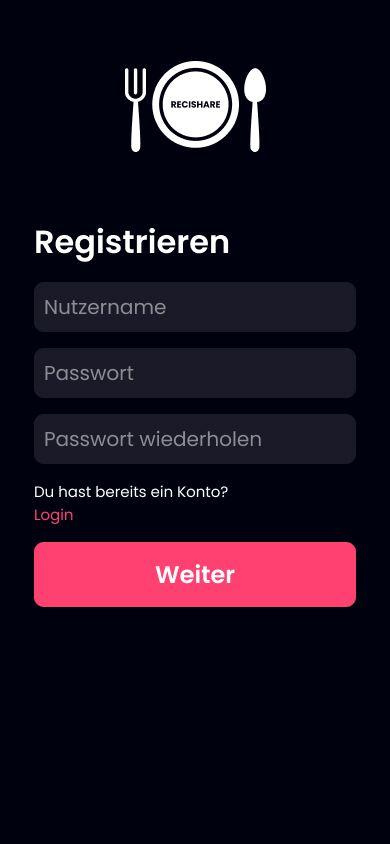
\includegraphics[height=80mm]{images/section7/RegisterView.jpg}
        \label{fig:A71}
        \caption{Registrierenansicht}
    \end{minipage}
    \begin{minipage}
        [t]{0.5\textwidth}
        \centering
        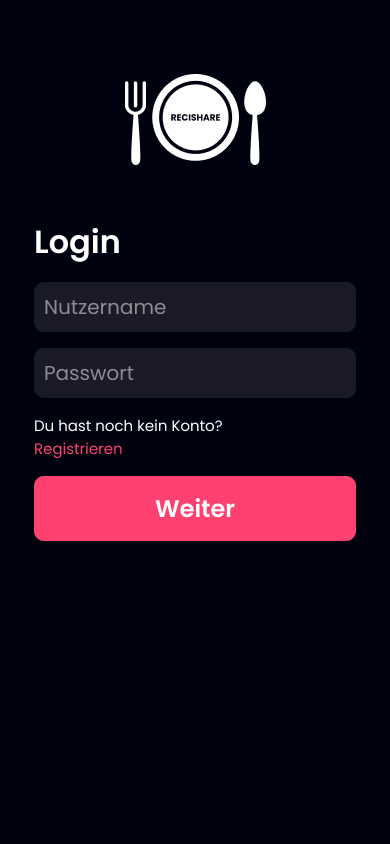
\includegraphics[height=80mm]{images/section7/LoginView.jpg}
        \label{fig:A72}
        \caption{Loginansicht}
    \end{minipage}
\end{figure}

\textbf{Gruppenansicht} $\langle$UI20$\rangle$

Auf der Gruppenansicht (\ref{fig:A73}) kann der Nutzer eine neue Gruppe erstellen, indem er den Namen der neuen Gruppe festlegt und auf "Weiter" drückt. Damit wird die Gruppe in der Datenbank angelegt und der Nutzer tritt dieser bei. Anschließend wird er auf die Hauptansicht $\langle$UI30$\rangle$ weitergeleitet. Alternativ kann der Nutzer auch einer bereits bestehenden Gruppe beitreten. Dazu muss er auf "Gruppe beitreten" drücken, woraufhin sich ein Popup-Fenster öffnet. Hier muss er den Gruppencode eingeben, den jede Gruppe besitzt. Existiert der Gruppencode, so wird der Nutzer der Gruppe hinzugefügt. Auch hier wird der Nutzer auf die Hauptansicht $\langle$UI30$\rangle$ weitergeleitet.

\begin{figure}[!htp]
    \centering
    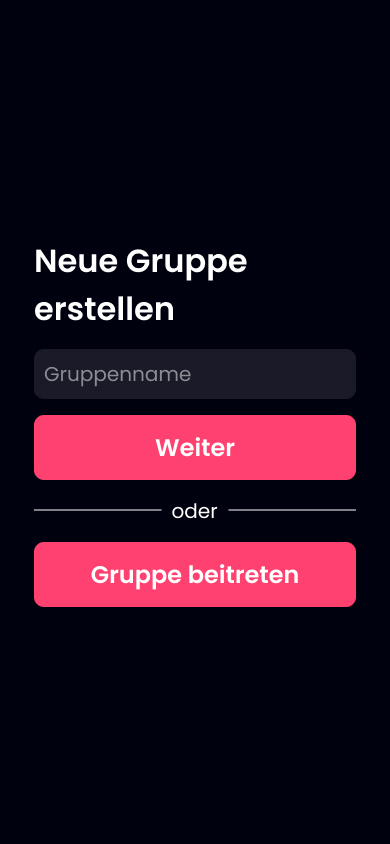
\includegraphics[height=80mm]{images/section7/GroupView.jpg}
    \label{fig:A73}
    \caption{Gruppenansicht}
\end{figure}
\newpage
\textbf{Hauptansicht} $\langle$UI30$\rangle$

In der Hauptansicht (\ref{fig:A74}) kann der Nutzer alle Rezepte aus den Gruppen, in denen er Mitglied ist sehen. Diese kann er nach verschiedenen Faktoren filtern und sortieren. Durch eine Suchleiste kann er außerdem schnell ein gewünschtes Rezept finden. Jedes Rezept wird hier mit Titel, dem ersten Bild, Kochdauer und Schwierigkeitsgrad abgebildet. Durch einen Klick auf das Herzsymbol wird ein Rezept zu den Favoriten hinzugefügt bzw. wieder entfernt. Klickt ein Nutzer auf ein Rezept, so gelangt er zur Rezeptansicht $\langle$UI40$\rangle$. Durch einen Klick auf das Notizblock-Symbol gelangt der Nutzer auf die Rezepterstellenansicht $\langle$UI60$\rangle$.

\begin{figure}[!htp]
    \centering
    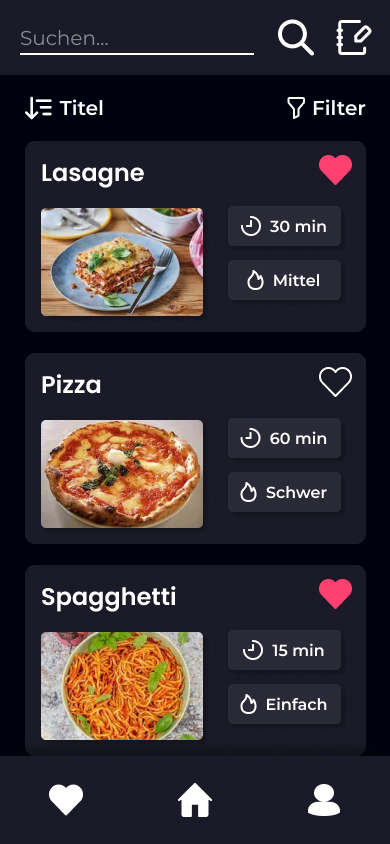
\includegraphics[height=80mm]{images/section7/MainView.jpg}
    \label{fig:A74}
    \caption{Hauptansicht}
\end{figure}

Unten am Bildschirm befindet sich eine Navigationsleiste, die es dem Nutzer ermöglicht, zwischen verschiedenen Ansichten zu wechseln. Durch einen Klick auf das Haus-Symbol gelangt der Nutzer auf die Hauptansicht $\langle$UI30$\rangle$. Durch einen Klick auf das Herz-Symbol gelangt der Nutzer auf die Favoritenansicht $\langle$UI50$\rangle$. Durch einen Klick auf das Personen-Symbol gelangt der Nutzer auf die Verwaltungsansicht $\langle$UI80$\rangle$.

\textbf{Rezeptansicht} $\langle$UI40$\rangle$

In der Rezeptansicht (\ref{fig:A75}) wird ein bestimmtes Rezept angezeigt. Es werden Name, Bilder, Zutaten, Zubereitungsanweisungen, Kochdauer, Schwierigkeitsgrad, Autor und Erstellungsdatum angezeigt. Der Nutzer kann durch anpassen der Portionenzahl automatisch die Zutatenmengen errechnen lassen. Durch einen Klick auf das Herzsymbol wird ein Rezept zu den Favoriten hinzugefügt bzw. wieder entfernt. Ist der Nutzer der Autor des Rezepts, so wird oben ein Stiftsymbol angezeigt. Durch einen Klick auf dieses Symbol gelangt der Nutzer auf die Rezepterstellenansicht $\langle$UI60$\rangle$, die bereits mit dem Rezept befüllt ist. Dort kann er das Rezept bearbeiten. Mit Hilfe des Plus-Symbols über den Bildern kann ein Nutzer außerdem Bilder hochladen, die dann für alle Nutzer im Rezept einsehbar sind. Dies geschieht mit Hilfe des betriebssystemeigenen Dateimanagers. Unten am Bildschirm ist wieder die Navigationsleiste zu finden. Außerdem kann der Nutzer wieder zurück zur vorherigen Ansicht gelangen, indem er auf das Zurück-Symbol oben links klickt.

\begin{figure}[!htp]
    \centering
    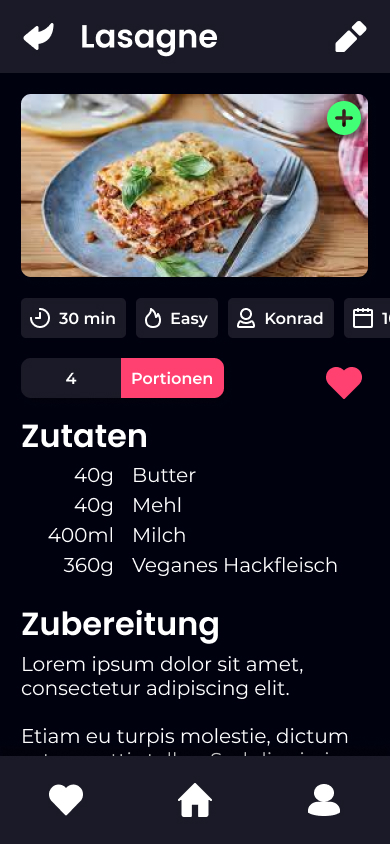
\includegraphics[height=80mm]{images/section7/RecipeView.jpg}
    \label{fig:A75}
    \caption{Rezeptansicht}
\end{figure}

\textbf{Favoritenansicht} $\langle$UI50$\rangle$

Die Favoritenansicht (\ref{fig:A76}) ist identisch zur Hauptansicht $\langle$UI30$\rangle$, nur dass hier nur die favorisierten Rezepte angezeigt werden. Außerdem gibt es hier keinen Button zum Rezepte erstellen.
\newpage
\begin{figure}[!htp]
    \centering
    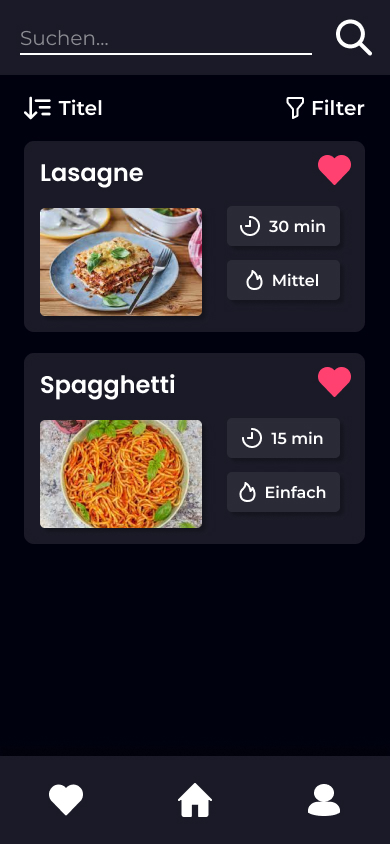
\includegraphics[height=80mm]{images/section7/FavouritesView.jpg}
    \label{fig:A76}
    \caption{Favoritenansicht}
\end{figure}

\textbf{Rezepterstellenansicht} $\langle$UI60$\rangle$

In dieser Ansicht (\ref{fig:A77}) kann ein Nutzer ein neues Rezept erstellen oder bearbeiten. Dazu gibt es verschiedene Eingabefelder, die der Nutzer ausfüllen kann. Diese umfassen den Rezeptnamen, Dauer und Schwierigkeitsgrad sowie die Zubereitungsanweisungen. Außerdem kann er Bilder mit Hilfe des betriebssystemeigenen Dateimanagers hochladen, indem er auf das Bild-Symbol klickt. 
Die Zutaten können mit einem Klick auf das Plus-Symbol hinzugefügt werden. Dazu öffnet sich die Zutatenauswahlansicht, in der der Nutzer die Zutat auswählen kann. Die bereits hinzugefügten Zutaten werden in einer Liste angezeigt und können durch einen Klick auf das Kreuz-Symbol entfernt werden. Ganz unten befindet sich ein Knopf zum Speichern des Rezepts. Durch einen Klick auf das Zurück-Symbol oben links gelangt der Nutzer zurück zur vorherigen Ansicht. Auch hier gibt es wieder die Navigationsleiste.

\begin{figure}[!htp]
    \centering
    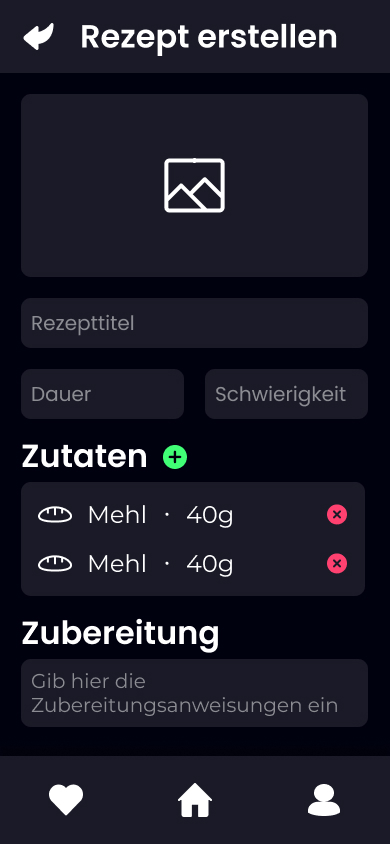
\includegraphics[height=80mm]{images/section7/RecipeCreationView.jpg}
    \label{fig:A77}
    \caption{Rezepterstellenansicht}
\end{figure}

\textbf{Zutatenauswahlansicht} $\langle$UI70$\rangle$

In dieser Ansicht (\ref{fig:A78}) kann der Nutzer Zutaten erstellen. Dazu schreibt er den Namen der Zutat in das Eingabefeld und wählt Einheit und Menge aus. Während der Nutzer die Zutat eingibt sollen automatisch Zutaten gesucht werden, die zum bisher geschriebenen Text passen und als Vorschlag unter dem Eingabefeld angezeigt werden. Durch Klick auf so einen Vorschlag wird der Zutatenname auf diesen Vorschlag gesetzt. Der Nutzer hat außerdem die Möglichkeit ein Icon für die Zutat aus einem Dropdownmenü zu wählen. Durch den "Hinzufügen"-Button wird die Zutat erstellt und der Nutzer gelangt zurück zur Rezepterstellenansicht $\langle$UI60$\rangle$.

\begin{figure}[!htp]
    \centering
    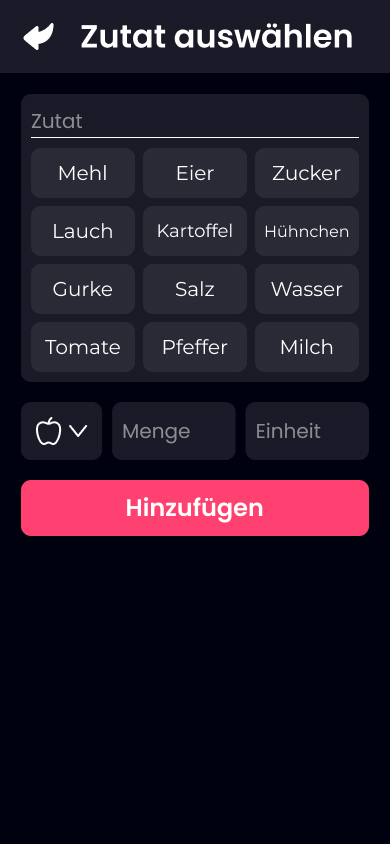
\includegraphics[height=80mm]{images/section7/IngredientPickerView.jpg}
    \label{fig:A78}
    \caption{Rezepterstellenansicht}
\end{figure}

\textbf{Verwaltungsansicht} $\langle$UI80$\rangle$

Die Verwaltungsansicht dient der Verwaltung des Nutzers und seiner Gruppen. Der Nutzer kann seinen Anzeigenamen ändern. Zudem kann er Gruppen austreten, in dem er auf das Kreuz-Symbol neben der entsprechenden Gruppe drückt. Außerdem kann er den Gruppencode mit Hilfe des Teilen-Symbols teilen. Durch das Plus-Symbol gelangt der Nutzer zur Gruppenansicht $\langle$UI90$\rangle$, in der er eine neue Gruppe erstellen kann oder einer bestehenden Gruppe beitritt. Außerdem sieht der Nutzer seine erstellten Rezepte, die er hier mit dem entsprechenden Button entfernen oder bearbeiten kann. Durch Klick auf das Rezept wird man zur entsprechenden Rezeptansicht $\langle$UI40$\rangle$. Mit dem Teilen-Button soll ein Rezept als PDF exportiert werden können.
Zudem kann der Nutzer sich ausloggen mit dem Symbol oben rechts. Daraufhin wird er zur Loginansicht $\langle$UI10$\rangle$weitergeleitet. Auch hier gibt es wieder die Navigationsleiste.

\begin{figure}[!htp]
    \centering
    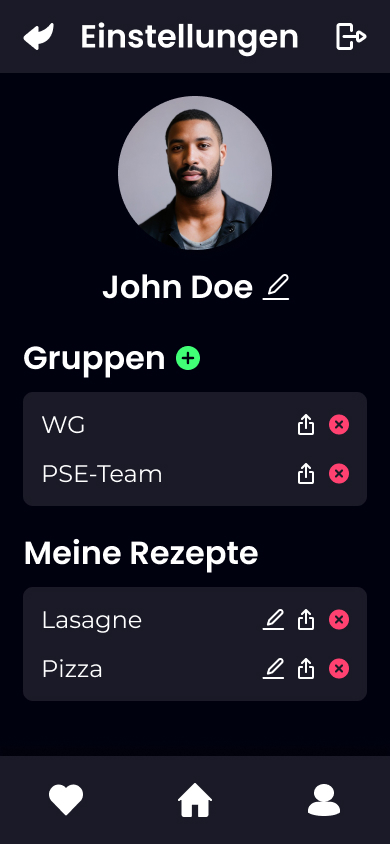
\includegraphics[height=80mm]{images/section7/SettingsView.jpg}
    \label{fig:A79}
    \caption{Verwaltungsansicht}
\end{figure}
\newpage
\section{Technische Produktumgebung}
In diesem Kapitel wird die technische Umgebung des Produktes beschrieben.

\subsection{Software}
\begin{itemize}
    \item Entwicklungsumgebung - Android Studio, IntelliJ
    \item Implementierungssprache der App - Dart
    \item Nuzterverwaltung - Firebase
    \item Client-Betriebssystem - Android 10 oder eine neuere Androidversion
    \item Implementierungssprache des Servers - ?
\end{itemize}

\subsection{Hardware}
\begin{itemize}
    \item Standard Smartphone mit Android Betriebssystem
\end{itemize}

\subsection{Produktschnittstellen}
Die Benutzerschnittstelle wird über ein GUI zur Verfügung gestellt.

\section{Glossar}

\end{document}
